\documentclass[journal,12pt,onecolumn]{IEEEtran}
\usepackage{cite}
\usepackage{graphicx}
\usepackage{amsmath,amssymb,amsfonts,amsthm}
\usepackage{algorithmic}
\usepackage{graphicx}
\usepackage{textcomp}
\usepackage{xcolor}
\usepackage{txfonts}
\usepackage{listings}
\usepackage{enumitem}
\usepackage{mathtools}
\usepackage{gensymb}
\usepackage{comment}
\usepackage[breaklinks=true]{hyperref}
\usepackage{tkz-euclide} 
\usepackage{listings}
\usepackage{gvv}                                        
%\def\inputGnumericTable{}                                 
\usepackage[latin1]{inputenc} 
\usetikzlibrary{arrows.meta, positioning}
\usepackage{xparse}
\usepackage{color}                                            
\usepackage{array}                                            
\usepackage{longtable}                                       
\usepackage{calc}                                             
\usepackage{multirow}
\usepackage{multicol}
\usepackage{hhline}                                           
\usepackage{ifthen}                                           
\usepackage{lscape}
\usepackage{tabularx}
\usepackage{array}
\usepackage{float}
\newtheorem{theorem}{Theorem}[section]
\newtheorem{problem}{Problem}
\newtheorem{proposition}{Proposition}[section]
\newtheorem{lemma}{Lemma}[section]
\newtheorem{corollary}[theorem]{Corollary}
\newtheorem{example}{Example}[section]
\newtheorem{definition}[problem]{Definition}
\newcommand{\BEQA}{\begin{eqnarray}}
\newcommand{\EEQA}{\end{eqnarray}}
\usepackage{float}
\theoremstyle{remark}
\usepackage{circuitikz}
\usepackage{tikz} 
\graphicspath{{figs/}}

\title{GATE 2024 STATISTICS}
\author{EE25BTECH11022 - SANKEERTHAN }
\date{}


\begin{document}
\maketitle
\textbf{\underline{General Aptitude}}

\begin{enumerate}
\item 
If ``$\rightarrow$'' denotes increasing order of intensity, then the meaning of the words  
[walk $\rightarrow$ jog $\rightarrow$ sprint] is analogous to [bothered $\rightarrow$ \underline{\phantom{imagine}} $\rightarrow$ daunted].  
Which one of the given options is appropriate to fill the blank?

\begin{enumerate}
\begin{multicols}{4}
\item phased
\item phrased
\item fazed
\item fused
\end{multicols}
\end{enumerate}
\hfill (GATE ST 2024)
\item 
Two wizards try to create a spell using all the four elements: water, air, fire, and earth.  
They decide to mix all these elements in \emph{all possible orders} and work independently.  
After exhausting all possible combinations, they conclude the spell does not work.  
How many attempts does each wizard make independently before concluding?


\begin{enumerate}
\begin{multicols}{4}
\item 24
\item 48
\item 16
\item 12
\end{multicols}
\end{enumerate}
\hfill (GATE ST 2024)
\item 
In an engineering college of $10,000$ students, $1500$ like neither their core branches nor other branches.  
The number of students who like their core branches is $\frac{1}{4}$ of those who like other branches.  
Number of students who like both core and other branches is $500$.  
The number of students who like their core branches is:

\begin{enumerate}
\begin{multicols}{4}
\item 1800
\item 3500
\item 1600
\item 1500
\end{multicols}
\end{enumerate}
\hfill (GATE ST 2024)
\item 
For positive non-zero real variables $x$ and $y$, if
$
\ln\brak{x + \frac{y}{2}}= \frac12\sbrak{ \ln\brak{x} + \ln\brak{y} }
$
then the value of $\frac{x}{y} + \frac{y}{x}$ is:

\begin{enumerate}
\begin{multicols}{4}
\item 1
\item $\frac12$
\item 2
\item 4
\end{multicols}
\end{enumerate}
\hfill (GATE ST 2024)
\item 
In the sequence $6, 9, 14, x, 30, 41$, a possible value of $x$ is:

\begin{enumerate}
\begin{multicols}{4}
\item 25
\item 21
\item 18
\item 20
\end{multicols}
\end{enumerate}
\hfill (GATE ST 2024)
\item 
Sequence the following sentences in a coherent passage.  
P: This fortuitous geological event generated a colossal amount of energy and heat that resulted in the rocks rising to an average height of $4\,\mathrm{km}$ across the contact zone.  
Q: Thus, the geophysicists tend to think of the Himalayas as an active geological event rather than as a static geological feature.  
R: The natural process of cooling of this massive edifice absorbed large quantities of atmospheric carbon dioxide, altering the Earth's atmosphere and making it better suited for life.  
S: Many millennia ago, a breakaway chunk of bedrock from the Antarctic Plate collided with the massive Eurasian Plate.

\begin{enumerate}
\begin{multicols}{4}
\item QPSR
\item QSPR
\item SPRQ
\item SRPQ
\end{multicols}
\end{enumerate}
\hfill (GATE ST 2024)
\item 
A person sold two different items at the same price.  
He made $10\%$ profit in one item, and $10\%$ loss in the other.  
Overall, the person made:

\begin{enumerate}
\begin{multicols}{4}
\item 1\% profit
\item 2\% profit
\item 1\% loss
\item 2\% loss
\end{multicols}
\end{enumerate}
\hfill (GATE ST 2024)
\item 
The pie charts show the shares of different power generation technologies in total electricity generation for years 2007 and 2023.

\begin{figure}
    \centering
    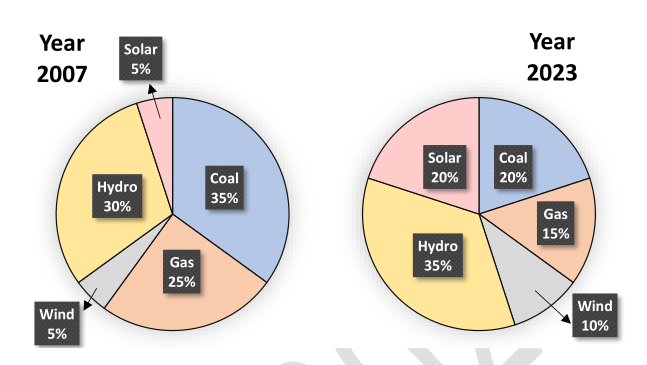
\includegraphics[width=0.5\columnwidth]{figs/1.png}
    \caption{}
    \label{fig:1}
\end{figure}
The renewable sources of electricity generation consist of Hydro, Solar and Wind. Assume total electricity generation is same for both years.  
Find the \% increase in renewable share from 2007 to 2023.

\begin{enumerate}
\begin{multicols}{4}
\item 25\%
\item 50\%
\item 77.5\%
\item 62.5\%
\end{multicols}
\end{enumerate}
\hfill (GATE ST 2024)
\item 
A cube is to be cut into $8$ equal pieces of identical size and shape.  
Each cut should be straight and extend fully through the cube.  
Minimum number of such cuts required is:

\begin{enumerate}
\begin{multicols}{4}
\item 3
\item 4
\item 7
\item 8
\end{multicols}
\end{enumerate}
\hfill (GATE ST 2024)
\item 
In the $4\times 4$ array below, each cell of the first three rows has either a cross (X) or a number.  
A number in a cell shows count of its immediate neighbours (adjacent or diagonal) \emph{not} having a cross.  
Given last row has no crosses, sum of four numbers to be filled in last row equals:


\begin{enumerate}
\begin{multicols}{4}
\item 11
\item 10
\item 12
\item 9
\end{multicols}
\end{enumerate}
\hfill (GATE ST 2024)

\item 
Let $D$ be the region bounded by the line $y = x$ and the parabola $y = 4x - x^2$. Then
$
\iint_{D} x \, dx \, dy
$
equals:

\begin{enumerate}
\begin{multicols}{4}
\item $\frac{27}{4}$
\item $\frac{29}{4}$
\item $7$
\item $6$
\end{multicols}
\end{enumerate}
\hfill (GATE ST 2024)
\item 
Let $\{a_n\}_{n \ge 1}$ be a sequence of real numbers such that $a_1 = \sqrt{6}$ and
$
a_{n+1} = \sqrt{6 + a_n}, \quad n \ge 1.
$
Consider the following statements:  
(I) $\{a_n\}_{n \ge 1}$ is an increasing sequence.  
(II) $\lim_{n \to \infty} a_n = 2$.

Which of the above statements is/are true?

\begin{enumerate}
\begin{multicols}{4}
\item Only (I)
\item Only (II)
\item Both (I) and (II)
\item Neither (I) nor (II)
\end{multicols}
\end{enumerate}
\hfill (GATE ST 2024)
\item 
Let $A$ be a $3 \times 3$ real matrix and $I_3$ be the $3 \times 3$ identity matrix.  
Which of the following statements is NOT true?

\begin{enumerate}

\item If the row-reduced echelon form of $A$ is $I_3$, then zero is not an eigenvalue of $A$
\item If zero is not an eigenvalue of $A$, then the row-reduced echelon form of $A$ is $I_3$
\item If $A$ has three distinct eigenvalues, then the row-reduced echelon form of $A$ is $I_3$
\item If the system $A \mathbf{x} = \mathbf{b}$ has a solution for every $3\times 1$ real vector $\mathbf{b}$, then the row-reduced echelon form of $A$ is $I_3$
\end{enumerate}
\hfill (GATE ST 2024)
\item 
Let $\mathbf{u}_1, \mathbf{u}_2, \mathbf{u}_3, \mathbf{v}_1, \mathbf{v}_2, \mathbf{v}_3$ be vectors in $\mathbb{R}^4$. Let $U$ be the span of $\{\mathbf{u}_1, \mathbf{u}_2, \mathbf{u}_3\}$ and $V$ be the span of $\{\mathbf{v}_1, \mathbf{v}_2, \mathbf{v}_3\}$.  

Statements:  
(I) If $\dim\brak{U \cap V} = 2$ and $\dim\brak{U} = 3$, then $\cbrak{\mathbf{v}_1, \mathbf{v}_2, \mathbf{v}_3}$ is linearly dependent.  
(II) If $U + V = \mathbb{R}^4$, then either $\brak{\mathbf{u}_1, \mathbf{u}_2, \mathbf{u}_3}$ is linearly independent or $\brak{\mathbf{v}_1, \mathbf{v}_2, \mathbf{v}_3}$ is linearly independent.

Which is/are true?

\begin{enumerate}
\begin{multicols}{4}
\item Only (I)
\item Only (II)
\item Both (I) and (II)
\item Neither (I) nor (II)
\end{multicols}
\end{enumerate}
\hfill (GATE ST 2024)
\item 
Consider $\mathbb{R}^2$ with standard inner product. If $\mathbf{u} = \myvec{ a \\ b }$ is such that  
$\langle \mathbf{u}, \myvec{ 1 \\ 2 } \rangle = 2$  
and  
$\langle \mathbf{u}, \myvec{ 4 \\ -2 } \rangle = -1$,  
then which statement is true?

\begin{enumerate}
\begin{multicols}{4}
\item $\langle \mathbf{u}, \myvec{ 1 \\ -1 } \rangle = \frac12$
\item $\langle \mathbf{u}, \myvec{ -1 \\ 1 } \rangle = \frac35$
\item $\langle \mathbf{u}, \myvec{ 2 \\ -\frac12 } \rangle = -\frac65$
\item $\langle \mathbf{u}, \myvec{ -\frac12 \\ 1 } \rangle = \frac45$
\end{multicols}
\end{enumerate}
\hfill (GATE ST 2024)
\item 
Let $A = \myvec{ a_1 & a_2 & a_3 \\ b_1 & b_2 & b_3 }$ be a $2\times 3$ real matrix with $\brak{a_1,a_2,a_3} \neq \brak{0,0,0}$, $\brak{b_1,b_2,b_3} \neq \brak{0,0,0}$, and $\mathrm{rank}\brak{A} = 1$.  
Define:  
$W = \cbrak{ \mathbf{x} \in \mathbb{R}^3 : A\mathbf{x} = \mathbf{0} }$  
$W_1 = \brak{ \mathbf{x} \in \mathbb{R}^3 : a_1 x_1 + a_2 x_2 + a_3 x_3 = 0}$ 
$W_2 = \brak{\mathbf{x} \in \mathbb{R}^3 : b_1 x_1 + b_2 x_2 + b_3 x_3 = 0}$

Statements:  
(I) $W = W_1 \cap W_2$  
(II) $W_1 = W_2$

Which is/are true?

\begin{enumerate}
\begin{multicols}{4}
\item Only (I)
\item Only (II)
\item Both (I) and (II)
\item Neither (I) nor (II)
\end{multicols}
\end{enumerate}
\hfill (GATE ST 2024)
\item 
Let $X$ take values $1$ and $2$. Let $M_X\brak{\cdot}$ be its moment generating function. If $E\brak{x} = \frac{10}{7}$, then the fourth derivative of $M_X\brak{\cdot}$ at $0$ equals:

\begin{enumerate}
\begin{multicols}{4}
\item $\frac{52}{7}$
\item $\frac{67}{7}$
\item $\frac{48}{7}$
\item $\frac{60}{7}$
\end{multicols}
\end{enumerate}
\hfill (GATE ST 2024)
\item 
Two fair dice (red and blue) are tossed. Let $A$ = red die shows $5$ or $6$.  
Let $B$ = sum of outcomes = 7.  
Let $C$ = sum of outcomes = 8.  
Which is true?

\begin{enumerate}
\item $A$ and $B$ are independent, and $A$ and $C$ are independent
\item $A$ and $B$ are independent, but $A$ and $C$ are not
\item $A$ and $C$ are independent, but $A$ and $B$ are not
\item Neither $A$ and $B$ nor $A$ and $C$ are independent
\end{enumerate}
\hfill (GATE ST 2024)
\item 
Let $X$ have PDF
$
f\brak{x} = \frac{\Gamma\brak{\alpha+\beta}}{\Gamma\brak{\alpha}\Gamma\brak{\beta}} x^{\alpha-1} \brak{1-x}^{\beta-1},\quad 0<x<1
$
where $\alpha>0$, $\beta>0$. If $E\brak{X} = \frac13$ and $E\brak{X^2} = \frac16$, then $\alpha + 3\beta =$:

\begin{enumerate}
\begin{multicols}{4}
\item 7
\item 5
\item 4
\item 8
\end{multicols}
\end{enumerate}
\hfill (GATE ST 2024)
\item 
Let $X$ and $Y$ have CDFs $F_X\brak{\cdot}$ and $F_Y\brak{\cdot}$. Which is NOT true?

\begin{enumerate}
\item There exist $X,Y$ with $F_X(u) = F_Y(u)$ for all $u\in\mathbb{R}$ and $P(X \neq Y) > 0$
\item There exist $X,Y$ with $F_X(u) = F_Y(u)$ for all $u\in\mathbb{R}$ and $P\brak{X = Y} = 0$
\item If $X$ and $Y$ are independent then $X^2$ and $Y^2$ are independent
\item If $X^2$ and $Y^2$ are independent then $X$ and $Y$ are independent
\end{enumerate}
\hfill (GATE ST 2024)
\item 
Let $\brak{F_n}_{n\ge1}$ be a sequence of cumulative distribution functions given by
$
F_n\brak{x} =
0, x < \--n, \\
\frac{x+n}{2n},  \--n \le x < n, \\
1, x \ge n.
$
Which statement is true?

\begin{enumerate}
\item $F_n\brak{x}$ converges for all $x\in\mathbb{R}$ and the limiting function is a CDF
\item $F_n\brak{x}$ converges for all $x\in\mathbb{R}$, but the limiting function is not a CDF
\item $F_n\brak{x}$ does not converge for any $x\in\mathbb{R}$
\item There exist $x,y\in\mathbb{R}$ such that $F_n\brak{x}$ converges but $F_n(y)$ does not
\end{enumerate}
\hfill (GATE ST 2024)
\item 
Let $\{W\brak{t}\}_{t\ge 0}$ be a standard Brownian motion. Which one is \textbf{NOT} true?

\begin{enumerate}
\begin{multicols}{4}
\item $E[w\brak{7}] = 0$
\item $E[w\brak{5}w\brak{9}] = 7$
\item $2w\brak{1}$ is $\mathcal{N}\brak{0,4}$
\item $E[w\brak{5} \mid w\brak{3} = 3] = 3$
\end{multicols}
\end{enumerate}
\hfill (GATE ST 2024)
\item 
Let $X_1, X_2, X_3$ be i.i.d. $\mathrm{Binomial}(n=100, p)$ random variables, with $p\in\brak{0,1}$ unknown. Define
$
T_1 = \brak{X_1 + X_2, X_3}, \quad T_2 = X_1 + X_2 + X_3.
$
Consider:  
(I) Distribution of $T_2$ given $T_1 = t_1$ is independent of $p$  
(II) Distribution of $T_1$ given $T_2 = t_2$ is independent of $p$

\begin{enumerate}
\begin{multicols}{4}
\item Only (I)
\item Only (II)
\item Both (I) and (II)
\item Neither (I) nor (II)
\end{multicols}
\end{enumerate}
\hfill (GATE ST 2024)
\item 
Let $X_1,\dots,X_n$ be a random sample from
$
f\brak{x;\theta} =
\theta \brak{2x}^{\theta-1},  0 < x \le \frac12, \\
\theta \brak{2 - 2x}^{\theta-1},  \frac12 < x \le 1, \\
0,  \text{otherwise},
$
where $\theta>0$. Which is an MLE of $\theta$?

\begin{enumerate}
\item $ n\sbrak{ \sum_{i:X_i\le 1/2} \log_e\brak{2X_i} + \sum_{i:X_i>1/2} \log_e\brak{2-2X_i} }^{-1}$
\item $ -n\sbrak{ \sum_{i:X_i\le 1/2} \log_e\brak{2X_i} + \sum_{i:X_i>1/2} \log_e\brak{2-2X_i} }^{-1}$
\item $ n\sbrak{ \sum_{i=1}^n \log_e\brak{2X_i} + \sum_{i=1}^n \log_e\brak{2-2X_i} }^{-1}$
\item $ -n\sbrak{ \sum_{i=1}^n \log_e\brak{2X_i} + \sum_{i=1}^n \log_e\brak{2-2X_i} }^{-1}$
\end{enumerate}
\hfill (GATE ST 2024)
\item 
In hypothesis testing, which statement is true?

\begin{enumerate}
\item Type-I error probability cannot be higher than Type-II error probability
\item Type-II error occurs when the test accepts $H_0$ when $H_0$ is false
\item Type-I error occurs when the test rejects $H_0$ when $H_0$ is false
\item Sum of probabilities of Type-I and Type-II errors must be 1

\end{enumerate}
\hfill (GATE ST 2024)
\item
A sample of size $n=40$ from 4 categories has:

\begin{tabular}{|c|c|c|c|c|}
\hline
Category & 1 & 2 & 3 & 4 \\ 
\hline
Observed Freq & 5 & 8 & 12 & 15 \\
\hline
\end{tabular}


Test $H_0:\ \theta_i = \frac14$ for all $i$ using $\chi^2$ GOF test. Which statement is true?

\begin{enumerate}
\begin{multicols}{2}
\item d.f. $=3$, test statistic $=5.8$
\item d.f. $=3$, test statistic $=1.4$
\item d.f. $=4$, test statistic $=5.8$
\item d.f. $=4$, test statistic $=1.4$
\end{multicols}
\end{enumerate}
\hfill (GATE ST 2024)
\item
Let $X_1,\dots,X_n$ be i.i.d. from a continuous distribution having unknown median $M$. Test $H_0: M=10$ vs $H_1: M>10$ at level $\alpha$ using $T =$ number of observations $>10$. If $t_0$ is observed $T$, then $p$-value is:

\begin{enumerate}
\begin{multicols}{4}
\item $ \sum_{i=t_0}^n \binom{n}{i} \brak{0.5}^n$
\item $ \sum_{i=10}^n \binom{n}{i} \brak{0.5}^n$
\item $ \sum_{i=0}^{10} \binom{n}{i} \brak{0.5}^n$
\item $ \sum_{i=0}^{t_0} \binom{n}{i} \brak{0.5}^n$
\end{multicols}
\end{enumerate}
\hfill (GATE ST 2024)
\item
Consider $y_i = \beta_0 + \beta_1 x_i + \epsilon_i$, $\epsilon_i$ i.i.d. mean 0, variance $\sigma^2$. Let $\bar{y}$ be sample mean, $\hat{\beta}_1$ LSE. Which is true?

\begin{enumerate}
\begin{multicols}{2}
\item $Cov\brak{\bar{y},\hat{\beta}_1} < 0$
\item $Cov\brak{\bar{y},\hat{\beta}_1} > 0$
\item $Cov\brak{\bar{y},\hat{\beta}_1} = 0$
\item $Cov\brak{\bar{y},\hat{\beta}_1}$ does not exist
\end{multicols}
\end{enumerate}
\hfill (GATE ST 2024)
\item
Consider same linear model as Q.28 but with statistics:
$
T_1 = \frac{1}{n-2}\sum_{i=1}^n (y_i - \hat{y}_i)^2,\quad
T_2 = \sum_{i=1}^n (\hat{y}_i - \bar{y})^2
$
Which is true?

\begin{enumerate}
\begin{multicols}{2}
\item Both $T_1$ and $T_2$ are unbiased estimators of $\sigma^2$
\item $T_1$ unbiased, $T_2$ not
\item $T_1$ not unbiased, $T_2$ unbiased
\item Neither is unbiased
\end{multicols}
\end{enumerate}
\hfill (GATE ST 2024)
\item
Power series $\sum_{n=0}^\infty a_n x^n$ with $a_{2n+1} = \frac{1}{2^{2n+1}}$, $a_{2n} = \frac{1}{3^{2n}}$ has radius of convergence equal to \_\_\_ (integer).
\item
Let $X$ be a random variable having $\mathrm{Poisson}\brak{\lambda}$ distribution with $\lambda > 0$ such that $P\brak{X=4} = 2P\brak{X=5}$.  
If $p_k = P\brak{X=k}$ for $k = 0,1,2,\dots$, and $p_\alpha = \max_{k} p_k$, then $\alpha =$ \underline{\phantom{imagine}} (integer).
\hfill (GATE ST 2024)
\item
Let $X_1, X_2, X_3$ be i.i.d. random variables with PDF
$
f\brak{x} = 
2x,  0 < x < 1, \\
0,  \text{otherwise}.
$
Then $P\brak{\min\cbrak{X_1,X_2,X_3}} \ge E\brak{X_1} =$ \underline{\phantom{imagine}} (round to two decimal places).
\hfill (GATE ST 2024)
\item
Let $\brak{x,y}$ have a bivariate normal distribution with $E\brak{x}=E\brak{Y}=0$. Let $\mathrm{Var}\brak{X \mid Y=1}$ be the conditional variance of $X$ given $Y=1$ and similarly for $\mathrm{Var}\brak{Y \mid X=2}$.  
If
$
\frac{E\brak{Y \mid X=2}}{E\brak{X \mid Y=1}} = 8,
$
then
$
\frac{\mathrm{Var}(Y \mid X=2)}{\mathrm{Var}(X \mid Y=1)} =
$
\underline{\phantom{imagine}} (integer).
\hfill (GATE ST 2024)
\item
Let $X$ be a random sample of size one from $N{0,\sigma^2}$ with $\sigma>0$ unknown. Let $\Phi\brak{\cdot}$ be the CDF of $\mathcal{N}\brak{0,1}$. Let $\chi^2_{\nu,\alpha}$ be the $\brak{1-\alpha}$-quantile of the central chi-square with $\nu$ degrees of freedom.  
Given: $\Phi\brak{1.96}=0.975$, $\Phi\brak{1.64}=0.95$, $\chi^2_{1,0.05} = 3.841$, $\chi^2_{2,0.05} = 5.991$.  
Test $H_0: \sigma^2=1$ vs $H_1: \sigma^2=2$ using NP most powerful test of size $0.05$: reject when $\lambda\brak{x} > c$, where  
$
\lambda\brak{x} = \frac{f\brak{x; \sigma^2=2}}{f\brak{x; \sigma^2=1}}.
$
Find $c =$ \underline{\phantom{imagine}} (round to two decimal places).
\hfill (GATE ST 2024)
\item
Linear regression: $y_i = \beta_1 x_i + \epsilon_i$, $i=1,\dots,n$, with $\beta_1$ unknown, $\epsilon_i$ uncorrelated mean 0, variance $\sigma^2>0$. 5 data points:  
$\brak{x_1,y_1}=\brak{2,5}$, $\brak{x_2,y_2}=\brak{1,6}$, $\brak{x_3,y_3}=\brak{3,4}$, $\brak{x_4,y_4}=\brak{2,3}$, $\brak{x_5,y_5}=\brak{4,6}$.  
LSE of $\beta_1 =$ \underline{\phantom{imagine}} (round to two decimal places).

\hfill (GATE ST 2024)
\item
$f:\mathbb{R}^2\to\mathbb{R}$ given by:
$
f\brak{x,y} = 108xy - 2x^2y - 2xy^2.
$
Which is NOT true?

\begin{enumerate}
\begin{multicols}{2}
\item $f$ has four critical points
\item $f$ has a local minimum at $\brak{0,0}$
\item $f$ has a local maximum at $\brak{18,18}$
\item $f$ has two or more saddle points
\end{multicols}
\end{enumerate}
\hfill (GATE ST 2024)
\item
$f:\mathbb{R}^2\to\mathbb{R}$ given by:
$
f\brak{x,y} = 
\frac{x^3 - y^3}{x^2 + y^2},  \brak{x,y} \neq \brak{0,0} \\
0,  \brak{x,y} = \brak{0,0}
$
Let $f_x$ and $f_y$ denote partial derivatives. Which is NOT true?

\begin{enumerate}
\begin{multicols}{2}
\item $f$ is continuous at $\brak{0,0}$
\item $f_x\brak{0,0} \neq f_y\brak{0,0}$
\item $f_x$ is continuous at $\brak{0,0}$
\item $f_y$ is not continuous at $\brak{0,0}$
\end{multicols}
\end{enumerate}
\hfill (GATE ST 2024)
\item
$X$ has PDF:
$
f\brak{x} = 
\frac{3}{8}\brak{x+1}^2,  -1 < x < 1, \\
0,  \text{otherwise}.
$
If $Y = 1 - X^2$, find $P\brak{Y \le 3/4}$.

\begin{enumerate}
\begin{multicols}{4}
\item $\frac{19}{32}$
\item $\frac{9}{16}$
\item $\frac{15}{32}$
\item $\frac{5}{8}$
\end{multicols}
\end{enumerate}
\hfill (GATE ST 2024)
\item
$X$ has PDF:
$
f\brak{x} = 
\frac{c_1}{\sqrt{x}},  0 < x \le 1, \\
\frac{c_2}{x^2},  1 < x < \infty, \\
0,  \text{otherwise},
$
where $c_1,c_2$ are constants. If $P\brak{X \in \sbrak{1/4, 4}} = 5/8$,  
consider:  
(I) $P\brak{X \in \sbrak{3,5}} = 1/12$  
(II) Both $X$ and $1/X$ do not have finite expectations.  
Which are true?

\begin{enumerate}
\begin{multicols}{4}
\item Only (I)
\item Only (II)
\item Both (I) and (II)
\item Neither (I) nor (II)
\end{multicols}
\end{enumerate}
\hfill (GATE ST 2024)
\item
Checkout counter service time $T$ (in minutes) has PDF:
$
f\brak{t} = 
\frac{1}{10} e^{-t/10},  t \ge 0, \\
0,  \text{otherwise}.
$
On arrival, you see 1 person in service for already 5 minutes. Assume independence of service times.  
Find $P\brak{\text{your total time} > 15}$.

\begin{enumerate}
\begin{multicols}{4}
\item $\frac{5}{2} e^{-3/2}$
\item $\frac{3}{2} e^{-3/2}$
\item $\frac{3}{2} e^{-5/2}$
\item $\frac{5}{2} e^{-5/2}$
\end{multicols}
\end{enumerate}
\hfill (GATE ST 2024)
\item
$X$ has a discrete uniform distribution on $\cbrak{1,3,5,\dots,99}$. Then
$E\brak{X \mid X  \text{is not a multiple of } 15}$ equals:

\begin{enumerate}
\begin{multicols}{4}
\item $ \frac{2365}{47}$
\item $ \frac{2365}{50}$
\item $50$
\item $47$
\end{multicols}
\end{enumerate}
\hfill (GATE ST 2024)
\item
Let $X_1,\dots,X_n$ be i.i.d. $\mathcal{N}\brak{\mu,\sigma^2}$, $\mu\in\mathbb{R}$, $\sigma>0$.  
Statements:
(I) If $\dfrac{\sqrt{5}}{\sigma\brak{2n+1}}\sum_{i=1}^n \brak{X_i-\mu} \sim \mathcal{N}\brak{0,1}$, then $n=2$.  
(II) $E\!\sbrak{ \big(-\log_e \Phi\big(\frac{X_1-\mu}{\sigma}\big)\big)^3 } = 6$, where $\Phi\brak{\cdot}$ is CDF of $\mathcal{N}\brak{0,1}$.

Which is/are true?

\begin{enumerate}
\begin{multicols}{4}
\item Only (I)
\item Only (II)
\item Both (I) and (II)
\item Neither (I) nor (II)
\end{multicols}
\end{enumerate}
\hfill (GATE ST 2024)
\item
Let $X_n$ be i.i.d. with PDF $f\brak{x} = e^{-(x-\theta)}$ for $x\ge\theta$, $\theta>0$.  
(I) $\frac{1}{n}\sum_{i=1}^n X_i \to_p \frac{\theta+1}{2}$ as $n\to\infty$.  
(II) $\lim_{n\to\infty}E\sbrak{\min\cbrak{X_1,\dots,X_n}} = \theta$.  

Which is/are true?

\begin{enumerate}
\begin{multicols}{4}
\item Only (I)
\item Only (II)
\item Both (I) and (II)
\item Neither (I) nor (II)
\end{multicols}
\end{enumerate}
\hfill (GATE ST 2024)
\item
Let $X_n\sim \text{Poisson}\brak{\lambda_n}$ where $\lambda_n = \lambda + \frac{1}{2n}$, $\lambda>0$. Which statement +is true?

\begin{enumerate}
\begin{multicols}{2}
\item $\frac1n\sum X_i$ is an unbiased estimator of $\lambda$
\item $\frac1n\sum X_i$ is a consistent estimator of $\lambda$
\item $\sum X_i$ is a consistent estimator of $\lambda$
\item $\frac1{n^2}\sum X_i$ is an unbiased estimator of $\lambda$
\end{multicols}
\end{enumerate}
\hfill (GATE ST 2024)
\item
Let $\mathbf{X}_1,\dots,\mathbf{X}_{25} \stackrel{i.i.d.}{\sim} N_3\brak{\mu,\Sigma}$, $\Sigma$ nonsingular unknown.  
Let $S = \frac1{24}\sum_{j=1}^{25} \brak{\mathbf{X_j} - \bar{\mathbf{X}}} \brak{\mathbf{X_j} - \bar{\mathbf{X}}}^\top$, and  
$B = \myvec{ 1 & 2 & 3 \\ -1 & 0 & 1 }$.  
Which is true?

\begin{enumerate}
\begin{multicols}{2}
\item $24B S B^\top$ is Wishart of order 3, df=24
\item $24B S B^\top$ is Wishart of order 2, df=25
\item $24B S B^\top$ is Wishart of order 2, df=24
\item $24B S B^\top$ is Wishart of order 3, df=25
\end{multicols}
\end{enumerate}
\hfill (GATE ST 2024)
\item
Regression $y_i = \beta_0 + \beta_1 x_i + \epsilon_i$, $\epsilon_i$ uncorrelated mean 0 var $\sigma^2$.  
Statements:  
(I) The 95\% joint confidence region for $\brak{\beta_0,\beta_1}$ is bounded by an ellipse.  
(II) Covariance between $\hat{\beta}_0$ and $\hat{\beta}_1$ does not involve $\sigma^2$.

Which is/are true?

\begin{enumerate}
\begin{multicols}{4}
\item Only (I)
\item Only (II)
\item Both (I) and (II)
\item Neither (I) nor (II)
\end{multicols}
\end{enumerate}
\hfill (GATE ST 2024)
\item
Let $f:\sbrak{-2,2}\to\mathbb{R}$ continuous. Which are true?

\begin{enumerate}
\item $F\brak{x} = \int_0^x f\brak{t}\,dt$ is differentiable on $(0,2)$
\item For any $x_1,\dots,x_{10}\in\sbrak{-2,2}$, there exists $x_0\in\sbrak{-2,2}$ such that $f(x_0) = \frac1{10}\sum_{i=1}^{10} f(x_i)$
\item $f$ is bounded on $\sbrak{-2,2}$
\item If $f$ differentiable at 0 and $f(0)=0$, then $\lim_{x\to0} \frac{f\brak{x}+f\brak{x^2}+\dots+f(\brak{x^{10}}}{x} = 10f'\brak{0}$
\end{enumerate}
\hfill (GATE ST 2024)
\item
Let $A$ be an $n\times n$ real matrix. Which are true?

\begin{enumerate}
\item If $A$ symmetri\hfill (GATE ST 2024)c and $A+\epsilon I_n$ PSD for all $\epsilon>0$, then $A$ is PSD  
\item If $n$ odd, then $A-A^\top$ not invertible  
\item If $A$ symmetric and all singular values $>0$, then $A$ positive definite  
\item If $1$ is the only singular value of $A$, then $A$ is orthogonal
\end{enumerate}
\hfill (GATE ST 2024)
\item
Which statements are true?

\begin{enumerate}
\item If $A$ is $3\times3$ real with 3 dis\hfill (GATE ST 2024)tinct eigenvalues, then $A$ is diagonalizable
\item If $A^2$ is diagonalizable, then $A$ is diagonalizable
\item For real $a,b,c$, if $\myvec{0&a&b\\0&0&c\\0&0&0}$ is diagonalizable, then $a=b=c=0$
\item If $A=\myvec{a&b&c\\0&d&e\\0&0&f}$ is diagonalizable, then $AA^\top = A^\top A$
\end{enumerate}
\hfill (GATE ST 2024)
\item
$\Omega=\sbrak{1,2,3,\dots}$. $\mathcal{H}$ all subsets of $\Omega$, $P\brak{k}) = 1/2^k$. Let $X\brak{\omega} = \omega$.

Which are true?
\begin{enumerate}
\item $\exists k$ with $P\brak{X=k} < 10^{-6}$
\item $\lim_{n\to\infty} P\brak{X \ge 4 + 1/n} = 1/16$
\item $\lim_{n\to\infty} P\brak{4 + 1/n^2 \le X < 5 - 1/n} = 1/16$
\item If $x_n = 3 + \brak{-1}^n/n$, then $\lim_{n\to\infty} P\brak{X \le x_n} = 7/8$
\end{enumerate}
\hfill (GATE ST 2024)
\item
Let $\brak{x,y}$ have joint PDF
$
f_{X,Y}\brak{x,y} =
\frac34,  x^2 \le y < 1,\ -1 \le x \le 1,\\
0,  \text{otherwise}.
$
Which statements are true?
\begin{enumerate}
\begin{multicols}{2}
\item $X$ has the same distribution as $-X$
\item $E\brak{Y \mid X=0} = \frac12$
\item $\mathrm{Corr}\brak{x,y} = 0$
\item $X$ and $Y$ are independent
\end{multicols}
\end{enumerate}
\hfill (GATE ST 2024)
\item
Let $\sbrak{X_n}_{n\ge 1}$ be independent with PDF
$
f_n\brak{x} =
\frac{1}{\lambda_n} e^{-x/\lambda_n}, x \ge 0,\\
0,  \text{otherwise},
$
where $\lambda_n = 10 - \sum_{i=1}^n \frac{5}{2^{i-1}}$.
Which statements are true?

\begin{enumerate}
\item $\cbrak{X_n}$ converges in distribution to the zero random variable
\item $\cbrak{X_n}$ converges in probability to the zero random variable
\item $\cbrak{X_n}$ converges in distribution to a Poisson$(10)$ random variable
\item $\cbrak{X_n}$ converges in probability to a Poisson$(10)$ random variable
\end{enumerate}
\hfill (GATE ST 2024)
\item
A Markov chain with state space $\brak{0,1,2}$ has transition matrix
$
\myvec{
\frac12 & \frac12 & 0 \\
\frac12 & \frac12 & 0 \\
\frac13 & \frac13 & \frac13
}.
$
Which statements are true?

\begin{enumerate}
\begin{multicols}{2}
\item $0$ and $1$ are recurrent
\item $2$ is transient
\item Chain has unique stationary distribution
\item Chain is irreducible
\end{multicols}
\end{enumerate}
\hfill (GATE ST 2024)
\item
Let $X_1,\dots,X_n$ be i.i.d.\ $\mathrm{Poisson}\brak{\lambda}$, $\lambda>0$ unknown.  
$T_1=\bar{X}$, $T_2 = \sqrt{\frac{1}{n-1} \sum \brak{X_i - \bar{X}}^2}$.
Which statements are true?

\begin{enumerate}
\begin{multicols}{2}
\item $T_1$ is unbiased for $\lambda$
\item $T_2$ is unbiased for $\sqrt{\lambda}$
\item $T_2^2$ is unbiased for $\lambda$
\item Both $T_1$ and $T_2$ estimate $\lambda$ and $\lambda^2$
\end{multicols}
\end{enumerate}
\hfill (GATE ST 2024)
\item
Bernoulli$\brak{p}$ sample $X_1,X_2,X_3$, $p\in\brak{0,1}$ unknown.
Define $T_1\brak{X_i,X_j,X_k} = X_i - X_j\brak{1 - X_k}$,  
$T_2\brak{X_i,X_j,X_k} = \frac12\brak{X_iX_j + X_jX_k}$.
Which statements are true?

\begin{enumerate}
\item $T_1\brak{X_1,X_2,X_3}$ has same distribution as $T_1\brak{X_2,X_3,X_1}$, but they may differ for realizations
\item $T_2\brak{X_1,X_2,X_3}$ and $T_2\brak{X_3,X_2,X_1}$ are both unbiased for $p^2$
\item $T_1\brak{\cdot}$ forms unbiased estimators for $p^2$ and always equal for cyclic permutations
\item $T_2\brak{X_1,X_2,X_3} = T_2\brak{X_3,X_2,X_1}$ for all realizations
\end{enumerate}
\hfill (GATE ST 2024)
\item
$X_1,\dots,X_n$ i.i.d.\ $\mathrm{Exp}\brak{\lambda}$, $\lambda>0$ unknown.  
$T_1 = \sum X_i$, $T_2 = 1/\sum X_i$.  
Testing $H_0: \lambda=\lambda_0$ vs $H_1: \lambda>\lambda_0$, which tests are UMP level $\alpha$?

\begin{enumerate}
\begin{multicols}{4}
\item Reject if $\frac{2}{\lambda_0} T_1 > \chi^2_{n,\alpha}$
\item Reject if $\frac{2}{\lambda_0} T_1 > \chi^2_{n,1-\alpha}$
\item Reject if $\frac{\lambda_0}{2} T_2 > \chi^2_{n,\alpha}$
\item Reject if $\frac{\lambda_0}{2} T_2 > \chi^2_{n,1-\alpha}$
\end{multicols}
\end{enumerate}
\hfill (GATE ST 2024)
\item
Two samples: $\cbrak{1,6,5,3}$ and $\cbrak{11,7,15,4}$. Mann\--Whitney $U_{MW}$ statistic has probabilities given:  
$P(U_{MW} > 12) \le 0.10$, $P(U_{MW}>14)\le 0.05$, $P(U_{MW}>15)\le 0.025$, $P(U_{MW}>16)\le 0.01$.  
Which statements are true?

\begin{enumerate}
\begin{multicols}{4}
\item $H_0$ rejected at $\alpha=0.10$
\item $H_0$ rejected at $\alpha=0.05$
\item $H_0$ rejected at $\alpha=0.025$
\item $H_0$ rejected at $\alpha=0.01$
\end{multicols}
\end{enumerate}
\hfill (GATE ST 2024)
\item
$\brak{X_1,X_2,X_3} \sim N_3(\mu,\Sigma)$ with $\mu =\sbrak{\,2,-3,1\,}^\top$ and  
$
\Sigma = \myvec{
25 & -2 & 4\\
-2 & 4 & 1\\
4 & 1 & 9 }
$
For which $\mathbf{a}$ are $X_2$ and $X_2 - \mathbf{a}^\top\sbrak{X_1,X_2}^\top$ independent?

\begin{enumerate}
\begin{multicols}{4}
\item $\myvec{0 \\1}$
\item $\myvec{-1 \\-1}$
\item $\myvec{0 \\2}$
\item $\myvec{2 \\2}$
\end{multicols}
\end{enumerate}
\hfill (GATE ST 2024)
\item
$A$ is $2\times2$ with $\mathrm{tr}\brak{A}=5$, $\det\brak{A}=6$. Let the characteristic polynomial of $\brak{A+I_2}^{-1}$ be $x^2 - b x + c$.  
Find $b/c =$ \underline{\phantom{imagine}} (integer).

\item
Markov chain, states $\cbrak{0,1,2}$, transition
$
\myvec{
0 & 1 & 0 \\
\frac12 & \frac14 & \frac14\\
\frac12 & \frac14 & \frac14
},
$
$P\brak{X_0=0} = P\brak{X_0=1} = \frac14$. Find $32\,E\brak{X_2} =$ \underline{\phantom{imagine}} (integer).
\hfill (GATE ST 2024)
\item
$\brak{x,y}$ has MGF
$
M_{X,Y}\brak{u,v} = \frac{e^{u^2/2}}{\brak{1-2v}^3},\quad v<\frac12.
$
Find $E\brak{ \frac{6X^2}{Y} } =$ \underline{\phantom{imagine}} \brak{2 decimals}.
\hfill (GATE ST 2024)
\item
$\cbrak{N\brak{t}}$ Poisson process with rate $\lambda$. Potholes at distances:  
$0.9, 1.3, 1.8, 2.7, 3.4, 4.1, 4.7, 5.5, 6.2, 6.8, 7.4, 8.1, 8.9, 9.2, 9.7$.  
MoM estimate of $\lambda =$ \underline{\phantom{imagine}} \brak{2 decimals}.
\hfill (GATE ST 2024)
\item
Sample size $4$ from $\mathrm{U}\brak{0,\theta}$. Let $X_{\brak{4}}$ be max. Test $H_0: \theta=1$ vs $H_1: \theta=0.1$; reject if $X_{(4)}<0.3$. Let $p$ be Type-I error. Find $100p =$ \underline{\phantom{imagine}} \brak{2 decimals}.
\hfill (GATE ST 2024)
\item
Sample mean $0.16$ from size $4$ normal with unknown mean, variance $1$. $\Phi\brak{2.28}=0.989$, $\Phi\brak{1.96}=0.975$, $\Phi\brak{(1.64}=0.95$.  
LRT at $\alpha=0.05$ for $H_0:\mu=0$ vs $H_1:\mu\neq0$. Find power at $\bar{x}=0.16 =$ \underline{\phantom{imagine}} \brak{3 decimals}.
\hfill (GATE ST 2024)
\item
Multiple regression $y_i = \beta_0 + \beta_1 x_{1i} + \beta_2 x_{2i} + \varepsilon_i$, $n=25$. Test $H_0: \beta_1=\beta_2=0$ with  
$
F_0 = \frac{1}{1} \cdot \frac{R^2}{1-R^2}.
$
Reject if $F_0 > F_{\alpha,2,22}$. Given $F_{0.025,2,22}=4.38$, $F_{0.05,2,22}=3.44$.  
Find smallest $R^2$ to reject at $\alpha=0.05 =$ \hfill (GATE ST 2024)\underline{\phantom{imagine}} \brak{2 decimals}.
\hfill (GATE ST 2024)
\end{enumerate}


\end{document}
